\documentclass[UTF8,a4paper,11pt]{ctexart}
\usepackage[a4paper,top=2.4cm,bottom=2.2cm,left=2.35cm,right=2.35cm]{geometry}
\setmainfont{Times New Roman}
\usepackage{graphicx,booktabs,array,longtable,amsmath,amssymb,bm,mathtools}
\usepackage{caption,subcaption,float,xcolor,placeins,needspace,setspace,enumitem}
\usepackage[hidelinks]{hyperref}
\usepackage[nameinlink,noabbrev]{cleveref}

\setlength{\parindent}{2em}
\setlength{\parskip}{0pt}
\setlength{\emergencystretch}{2em}
\setstretch{1.12}

\captionsetup{font=small,labelfont=normalfont,labelsep=quad,justification=centering}
\ctexset{
  section={format=\centering\heiti\zihao{4},beforeskip=1.5ex,afterskip=1.2ex},
  subsection={format=\heiti\zihao{-4},beforeskip=1.2ex,afterskip=.6ex},
  subsubsection={format=\heiti\zihao{-4},beforeskip=.8ex,afterskip=.4ex}
}

\graphicspath{{figures/q2/}{../../figures/q2/}{../figures/q2/}}

\begin{document}
\songti\zihao{-4}
\pagestyle{plain}
\setcounter{section}{1}\setcounter{figure}{8}\setcounter{table}{5}

\section{问题二：缺失场景下的多模态情感预测模型}\label{sec:q2}

\subsection{问题分析与总体方案}\label{subsec:q2_plan}
本问研究文本、语音和视觉模态在局部连续区间发生缺失时的情感预测。附件2提供统一对齐的三模态序列，因此可在原始有效槽位上构造连续缺失，并分析缺失模态、缺失位置和缺失长度对极性分类与强度回归的影响。

本文选取均值池化、张量融合、低秩融合、时序记忆、跨模态注意力及缺失增强等结构进行适配比较，各方法统一使用相同输入接口、划分方式与双任务输出。

本文构建的模型由掩码均值池化（Masked Mean Pooling，MMP）基线与轻量时间注意力残差池化（Lightweight Temporal Attention Residual Pooling，LTARP）两部分组成。图~\ref{fig:q2_arch} 给出总体流程。对每个样本，三路模态首先分别进行聚合，形成文本、语音和视觉表示；三路表示拼接后经过共享融合层，分别由分类头输出消极、中性、积极三类情感极性，由回归头输出连续情感强度。完整输入与局部连续缺失输入沿用相同的网络结构与双任务预测设置。

\begin{figure}[htbp]\centering
\includegraphics[width=.94\textwidth]{{q2 架构图}.pdf}
\caption{LTARP的三模态双路池化与双任务预测流程。掩码均值和内容加权表示经同一模态映射、残差组合后进入融合层。}
\label{fig:q2_arch}\end{figure}

\subsection{数据表示与预测任务}\label{subsec:q2_data}
本问使用附件2提供的CMU-MOSEI对齐特征文件（\texttt{aligned-50.pkl}）。训练集、验证集和测试划分分别包含3395、728和727条样本。模型参数由训练集学习，网络结构与超参数由验证集确定，测试划分与无标签附件3不参与选模。

对齐特征序列的统一最大长度为$T=50$。样本$i$在文本、语音和视觉模态的输入矩阵分别表示为：
\begin{equation}
\mathbf X_i^{(T)} \in \mathbb R^{50 \times 768},\quad
\mathbf X_i^{(A)} \in \mathbb R^{50 \times 74},\quad
\mathbf X_i^{(V)} \in \mathbb R^{50 \times 35}.
\label{eq:q2_tensor_dim}
\end{equation}
设样本$i$的原始有效序列长度为$L_i$（$3 \le L_i \le 50$）。有效时序区间由随附的注意力掩码确定。定义槽位有效指示变量$p_{it}$：
\begin{equation}
p_{it} = \begin{cases}
1, & t \in \{1, 2, \dots, L_i\},\\
0, & t \in \{L_i+1, \dots, 50\}.
\end{cases}
\label{eq:q2_mask_def}
\end{equation}
原生零向量属于数据中的已有输入状态，仍按有效槽位参与模型计算。人工缺失则由实验协议将指定连续区间置零，两者在统计时分别记录。

真实连续情感强度标签记为$y_i \in [-3.0, +3.0]$。连续标签小于0、等于0和大于0分别对应消极、中性和积极：
\begin{equation}
c_i = \begin{cases}
0 \quad (\text{消极 Negative}), & y_i < 0,\\
1 \quad (\text{中性 Neutral}), & y_i = 0,\\
2 \quad (\text{积极 Positive}), & y_i > 0.
\end{cases}
\label{eq:q2_label_split}
\end{equation}
其中$y_i = 0$对应中性类。图~\ref{fig:q2_data} 给出样本划分规模、三类极性分布、连续强度标签密度及序列有效长度分布。

\begin{figure}[htbp]\centering
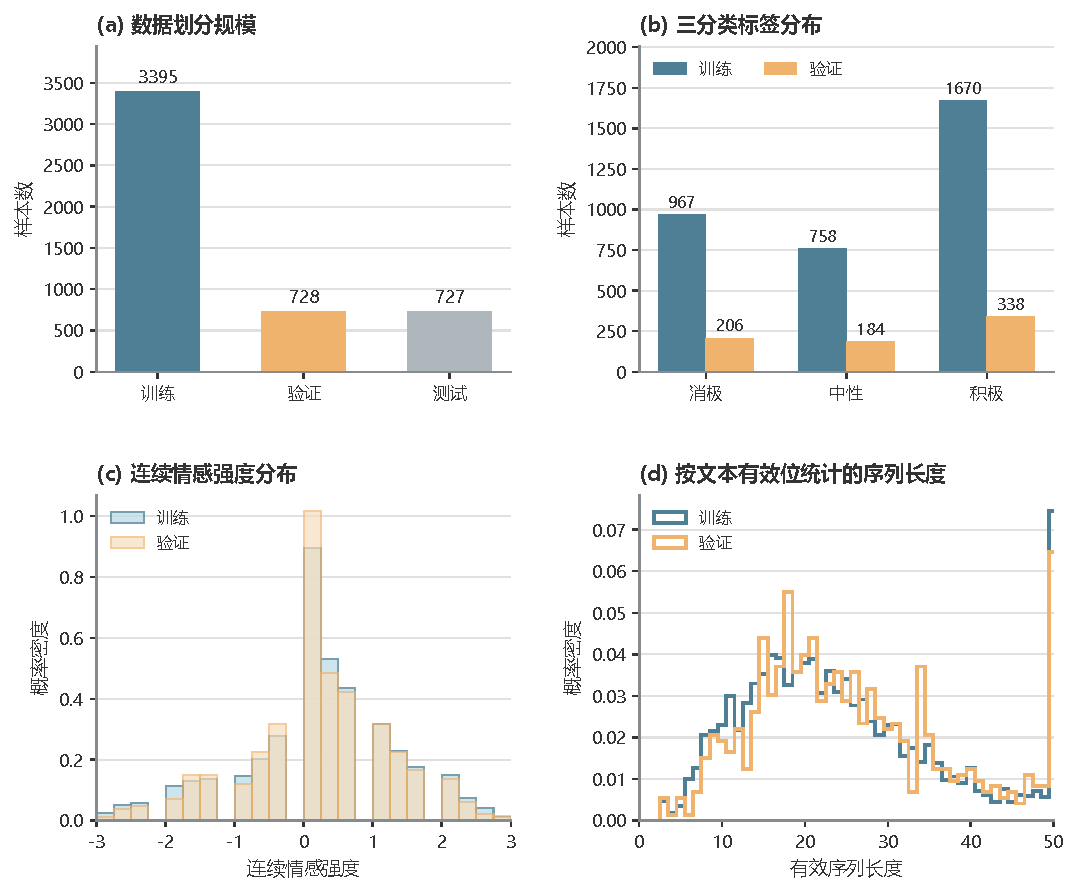
\includegraphics[width=.96\textwidth]{fig10_q2_data_statistics.pdf}
\caption{附件2 aligned-50特征的划分、类别、连续强度和有效长度分布。}
\label{fig:q2_data}\end{figure}
\FloatBarrier

基础性能采用四项标准指标评价：
\begin{itemize}[leftmargin=2.5em,itemsep=0pt,topsep=2pt]
  \item 准确率（Accuracy，$\uparrow$）：$\operatorname{Acc} = \frac{1}{N}\sum_{i=1}^N \mathbb I(\hat c_i = c_i)$；
  \item 宏平均F1（Macro-F1，$\uparrow$）：$\operatorname{MacroF1} = \frac{1}{3}\sum_{k=0}^2 \frac{2 \cdot \operatorname{Precision}_k \cdot \operatorname{Recall}_k}{\operatorname{Precision}_k + \operatorname{Recall}_k}$；
  \item 平均绝对误差（MAE，$\downarrow$）：$\operatorname{MAE} = \frac{1}{N}\sum_{i=1}^N |\hat y_i - y_i|$；
  \item 皮尔逊相关系数（Pearson，$r$，$\uparrow$）：$\operatorname{Pearson} = \frac{\sum_{i=1}^N (\hat y_i - \bar{\hat y})(y_i - \bar y)}{\sqrt{\sum_{i=1}^N (\hat y_i - \bar{\hat y})^2}\sqrt{\sum_{i=1}^N (y_i - \bar y)^2}}$。
\end{itemize}

\subsection{掩码均值池化基线}\label{subsec:q2_base}
MMP分别处理文本、语音和视觉序列。对样本$i$的模态$m \in \{T, A, V\}$，在有效指示位$p_{it}$约束下计算特征均值：
\begin{equation}
\boldsymbol\mu_i^{(m)} = \frac{\sum_{t=1}^{50} p_{it} \mathbf x_{it}^{(m)}}{\sum_{t=1}^{50} p_{it}}.
\label{eq:q2_mean_pool}
\end{equation}
均值向量通过模态专属映射$P_m(\cdot)$得到128维模态表示：
\begin{equation}
\mathbf h_{i,0}^{(m)} = P_m\left(\boldsymbol\mu_i^{(m)}\right) = \operatorname{Dropout}\Big(\operatorname{GELU}\big(\operatorname{LayerNorm}(\mathbf W_m \boldsymbol\mu_i^{(m)} + \mathbf b_m)\big)\Big).
\label{eq:q2_proj_layer}
\end{equation}
三路128维模态表示拼接为384维向量$\mathbf h_i^{\mathrm{concat}} = \big[\mathbf h_{i,0}^{(T)};\, \mathbf h_{i,0}^{(A)};\, \mathbf h_{i,0}^{(V)}\big]$，再经128维融合层得到联合表征$\mathbf z_i$：
\begin{equation}
\mathbf z_i = \operatorname{Dropout}\Big(\operatorname{GELU}\big(\operatorname{LayerNorm}(\mathbf W_f \mathbf h_i^{\mathrm{concat}} + \mathbf b_f)\big)\Big).
\end{equation}
联合表征分别连接三分类输出头和强度回归输出头：
\begin{equation}
\hat{\mathbf p}_i = \operatorname{Softmax}(\mathbf W_c \mathbf z_i + \mathbf b_c) \in \mathbb R^3,\qquad
\hat y_i = \mathbf W_r \mathbf z_i + b_r \in \mathbb R.
\label{eq:q2_heads}
\end{equation}
预测类别取最大概率对应项：$\hat c_i = \arg\max_{k \in \{0,1,2\}} \hat p_{ik}$。

训练集三类样本数分别为967、758和1670，因此分类损失采用类别频数逆加权交叉熵：
\begin{equation}
w_c = \frac{N_{\mathrm{train}}}{3 \cdot N_c},\qquad
\mathcal L_{\mathrm{WCE}} = -\frac{1}{N}\sum_{i=1}^N \sum_{k=0}^2 w_k \cdot \mathbb I(c_i = k) \log \hat p_{ik}.
\end{equation}
回归损失采用SmoothL1：
\begin{equation}
\mathcal L_{\mathrm{SmoothL1}} = \frac{1}{N}\sum_{i=1}^N \ell_{\mathrm{smooth}}(\hat y_i - y_i),\quad
\ell_{\mathrm{smooth}}(u) = \begin{cases}
0.5 u^2, & |u| < 1,\\
|u| - 0.5, & |u| \ge 1.
\end{cases}
\end{equation}
两者以相同权重相加：
\begin{equation}
\mathcal L = \mathcal L_{\mathrm{WCE}} + \lambda_r \mathcal L_{\mathrm{SmoothL1}},\qquad \lambda_r = 1.0.
\label{eq:q2_loss_full}
\end{equation}

MMP参数量为163460。输入直接采用附件2提供的原始数值特征，不额外进行标准化。优化器采用AdamW，学习率为$10^{-3}$，权重衰减为$10^{-4}$，批量大小为128，随机失活率为0.1。模型最多训练80轮，提前停止耐心轮数为12轮。基线在完整输入上训练，训练期连续遮挡方案的结果见消融实验。

\subsection{内容加权残差池化}\label{subsec:q2_pool}
MMP对有效槽位等权聚合。LTARP增加逐槽位标量打分器，根据当前槽位特征生成权重，并形成内容加权表示：
\begin{equation}
e_{it}^{(m)} = f_m(\mathbf x_{it}^{(m)}) = \mathbf w_{m,2}^\top \tanh(\mathbf W_{m,1} \mathbf x_{it}^{(m)} + \mathbf b_{m,1}) + b_{m,2}.
\end{equation}
权重在原始有效槽位内通过Softmax归一化：
\begin{equation}
\alpha_{it}^{(m)} = \frac{p_{it}\exp(e_{it}^{(m)})}{\sum_{s: p_{is}=1} \exp(e_{is}^{(m)})},\qquad
\mathbf a_i^{(m)} = \sum_{t=1}^{50} \alpha_{it}^{(m)} \mathbf x_{it}^{(m)}.
\label{eq:q2_alpha_softmax}
\end{equation}
填充位的$\alpha_{it}^{(m)}$恒为0。

LTARP令均值表示和内容加权表示共享$P_m$，并通过可学习系数$\gamma_m$相加：
\begin{equation}
\mathbf h_i^{(m)} = P_m\big(\boldsymbol\mu_i^{(m)}\big) + \gamma_m \cdot P_m\big(\mathbf a_i^{(m)}\big), \quad m \in \{T, A, V\}.
\label{eq:q2_residual_composite}
\end{equation}

训练分为两个阶段。第一阶段以 MMP 为完整基线进行训练，文本、语音和视觉三路模态映射 $P_T,P_A,P_V$、共享融合层以及分类、回归两个预测头同时更新。训练完成后保存对应检查点，并将其参数作为第二阶段 LTARP 的初始化参数。第二阶段保持上述基线参数不变，仅增加三个模态对应的内容打分器 $f_T,f_A,f_V$ 和三个残差系数 $\gamma_T,\gamma_A,\gamma_V$。由于 $\gamma_m$ 初值设为 0，第二阶段初始时模态输出为
\begin{equation}
\mathbf h_i^{(m)} = P_m(\boldsymbol\mu_i^{(m)}),
\end{equation}
随着训练进行，内容加权分支通过 $\gamma_m P_m(\mathbf a_i^{(m)})$ 逐步参与模态表示。第二阶段新增可训练参数共 883 个，其中三个模态打分器和三个残差系数共同更新，模型总参数量由 163460 增至 164343。

\subsection{连续缺失场景与评价协议}\label{subsec:q2_benchmark}
验证协议包含完整输入和54种局部连续缺失场景：
\begin{itemize}[leftmargin=2.5em,itemsep=0pt,topsep=2pt]
  \item 单模态场景集$\mathcal C_1$（45种）：选择单模态$m \in \{T, A, V\}$，目标比例$\mathcal R = \{0.1, 0.2, 0.3, 0.4, 0.5\}$，位置$\mathcal P = \{\mathrm{front}, \mathrm{middle}, \mathrm{rear}\}$，共$3 \times 5 \times 3 = 45$种；
  \item 双模态场景集$\mathcal C_2$（9种）：选择模态对$\{\{T, A\}, \{T, V\}, \{A, V\}\}$，固定$\rho_{\mathrm{target}} = 0.3$，取三个位置$\mathcal P$，共$3 \times 1 \times 3 = 9$种。
\end{itemize}

对有效长度为$L_i$的样本，遮挡槽位数与实际遮挡比例计算为：
\begin{equation}
\ell_i = \max\big(1,\, \operatorname{round}(\rho_{\mathrm{target}} \cdot L_i)\big),\qquad
\rho_{\mathrm{actual}, i} = \frac{\ell_i}{L_i}.
\label{eq:q2_mask_len}
\end{equation}
验证集728条样本中，$\rho_{\mathrm{target}} = 0.1$对应的实际遮挡比例范围为0.0714至0.3333（均值0.1040）；$\rho_{\mathrm{target}} = 0.5$对应的范围为0.4000至0.6667（均值0.5009）。由于 $\ell_i$ 必须取整数，相同的 $\rho_{\mathrm{target}}$ 在不同有效长度样本上对应不同的 $\rho_{\mathrm{actual},i}$。因此，后续图表中的横轴统一使用 $\rho_{\mathrm{target}}$ 标识实验条件，而样本实际缺失程度由 $\rho_{\mathrm{actual},i}$ 单独记录。对于短序列样本，至少遮挡 1 个有效槽位；对于较长序列，实际比例逐渐接近预设比例。

前段、中段、后段的起点索引$s_i$依次取$0$、$\lfloor (L_i - \ell_i)/2 \rfloor$和$L_i - \ell_i$。遮挡仅将指定模态在$[s_i, s_i + \ell_i - 1]$内的特征置零，其余模态及填充掩码保持原样。

验证期综合得分定义为：
\begin{equation}
S = \frac{1}{4}\operatorname{Acc} + \frac{1}{4}\operatorname{MacroF1} + \frac{1}{4}\left(1 - \frac{\operatorname{MAE}}{6}\right) + \frac{1}{8}(\operatorname{Pearson} + 1).
\label{eq:q2_score_s}
\end{equation}
跨场景综合分数定义为：
\begin{equation}
R = \frac{1}{2}\left(S_{\mathrm{clean}} + \frac{1}{54}\sum_{j=1}^{54} S_j\right).
\label{eq:q2_robust_r}
\end{equation}
本文使用$R$作为候选模型的综合选择指标。

对于每一种缺失配置，728 条验证样本均按照各自有效长度 $L_i$ 单独计算遮挡长度和起始位置，再统一完成整套验证集推理。每个场景分别得到 Accuracy、Macro-F1、MAE 和 Pearson 四项指标。设第 $s$ 个随机种子在第 $j$ 个缺失场景下某项指标为 $M_{s,j}$，则该种子的 54 场景平均值记为
\begin{equation}
\bar M_s = \frac{1}{54}\sum_{j=1}^{54}M_{s,j}, \qquad s\in\{42,43,44\}.
\end{equation}
三次独立训练结果再计算均值与样本标准差。图 11--14 中涉及跨场景汇总的结果均按照“先种子内汇总、再种子间统计”的顺序计算。

表6、表8和表9依据完整输入验证集$S_{\mathrm{clean}}$选择检查点；图11–14采用依据$R$选择的LTARP检查点。算法~1 给出54种缺失场景评测的执行流程。

\begin{table}[htbp]
\centering\small
\begin{tabular}{p{0.95\textwidth}}
\toprule
\textbf{算法 1} 多模态连续缺失基准评测算法\\
\midrule
\textbf{输入}：验证集多模态特征 $\{\mathbf X_i^{(T)}, \mathbf X_i^{(A)}, \mathbf X_i^{(V)}\}_{i=1}^N$，有效掩码 $\{p_{it}\}$，已选定模型 $\mathcal M$；\\
\textbf{输出}：完整输入指标、54种缺失场景指标及综合分数 $R$；\\
\textbf{步骤}：\\
1. 在完整输入上运行 $\mathcal M$，输出预测并计算 $\operatorname{Acc}_{\mathrm{clean}}, \operatorname{MacroF1}_{\mathrm{clean}}, \operatorname{MAE}_{\mathrm{clean}}, \operatorname{Pearson}_{\mathrm{clean}}$ 及 $S_{\mathrm{clean}}$；\\
2. 遍历54种缺失配置 $c = (\mathcal M_{\mathrm{target}}, \rho_{\mathrm{target}}, \mathrm{pos}) \in \mathcal C$：\\
\quad 2.1 对每个样本 $i = 1, \dots, N$：\\
\qquad a. 统计有效长度 $L_i = \sum_{t=1}^{50} p_{it}$；\\
\qquad b. 按式~\eqref{eq:q2_mask_len}计算 $\ell_i$；\\
\qquad c. 根据 $\mathrm{pos}$ 确定起点 $s_i$；\\
\qquad d. 将指定模态在区间 $[s_i, s_i + \ell_i - 1]$ 内的特征置零；\\
\quad 2.2 在当前受损特征上运行 $\mathcal M$，记录对应指标与得分 $S_j$；\\
3. 按式~\eqref{eq:q2_robust_r}计算54种场景平均值与综合分数 $R$。\\
\bottomrule
\end{tabular}
\end{table}

\subsection{基线与LTARP的结构比较}\label{subsec:q2_fair}
表~\ref{tab:q2_main} 在完整输入验证集选模规则下比较MMP与LTARP。数值为三个独立随机种子（42、43、44）的均值$\pm$样本标准差。

\begin{table}[htbp]
\centering\small\setlength{\tabcolsep}{4pt}
\caption{统一完整输入选模规则下的模型结构比较（三种子均值$\pm$样本标准差）}
\label{tab:q2_main}
\begin{tabular}{llcccc}
\toprule
条件 & 模型 & 准确率$\uparrow$ & 宏平均F1$\uparrow$ & MAE$\downarrow$ & 相关系数$\uparrow$\\
\midrule
完整输入 & MMP & $0.6401\pm0.0048$ & $0.6139\pm0.0091$ & $0.6079\pm0.0103$ & $0.6409\pm0.0043$\\
完整输入 & LTARP & $0.6415\pm0.0050$ & $0.6243\pm0.0026$ & $0.6052\pm0.0063$ & $0.6475\pm0.0024$\\
\addlinespace
54场景平均 & MMP & $0.6349\pm0.0062$ & $0.6092\pm0.0075$ & $0.6111\pm0.0098$ & $0.6359\pm0.0038$\\
54场景平均 & LTARP & $0.6334\pm0.0038$ & $0.6163\pm0.0013$ & $0.6086\pm0.0059$ & $0.6417\pm0.0024$\\
\bottomrule
\end{tabular}
\end{table}

完整输入下，LTARP相对MMP的准确率提高0.0014，宏平均F1提高0.0104，MAE降低0.0028，皮尔逊相关系数提高0.0066。

缺失场景平均下，LTARP的宏平均F1提高0.0071，MAE降低0.0026，相关系数提高0.0057，准确率降低0.0015。四项指标的变化方向并不完全一致。

三个随机种子的配对综合分数差（$\Delta R = R_{\mathrm{LTARP}} - R_{\mathrm{MMP}}$）分别为$+0.005600$、$+0.003791$和$-0.000090$，平均差值为$+0.003100 \pm 0.002907$。

\subsection{缺失类型、位置与相对时长}\label{subsec:q2_patterns}
图~\ref{fig:q2_ratio} 给出单模态遮挡比例实验结果。数据点先在同种子内对三个位置平均，再对三种子求均值与标准差。

\begin{figure}[htbp]\centering
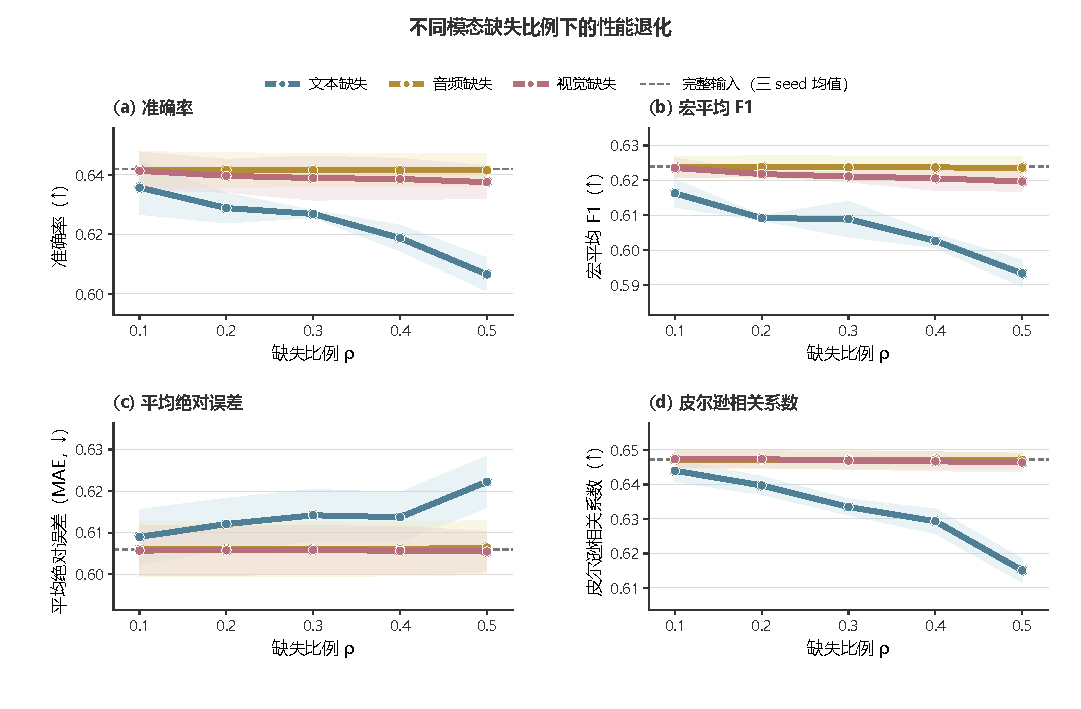
\includegraphics[width=.96\textwidth]{fig11_q2_modality_missing_degradation.pdf}
\caption{三种单模态在不同预设遮挡比例下的验证集性能。阴影为三个初始化之间的样本标准差；虚线为完整输入均值。}
\label{fig:q2_ratio}\end{figure}
\FloatBarrier

文本遮挡比例由0.1增至0.5时，Macro-F1由0.6163下降至0.5933，MAE由0.6090升至0.6222；语音和视觉的变化较小。在本实验设置下，文本遮挡造成的性能下降大于语音和视觉遮挡。

\begin{figure}[htbp]\centering
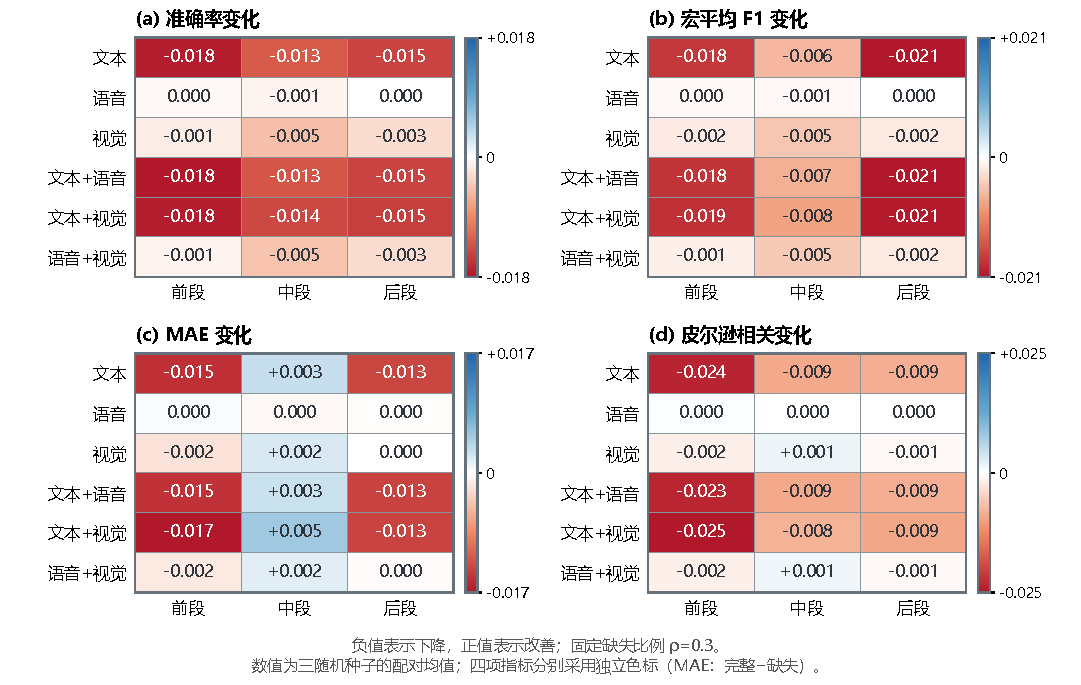
\includegraphics[width=.96\textwidth]{fig12_q2_modality_location_absolute_degradation.pdf}
\caption{目标比例0.3时各模态组合和遮挡位置相对于同种子完整输入的指标变化。正值表示退化；四项指标采用独立色标。}
\label{fig:q2_location}\end{figure}

在$\rho_{\mathrm{target}}=0.3$下，图~\ref{fig:q2_location} 给出各模态组合和遮挡位置相对于同种子完整输入的指标变化（正值表示退化）。文本前、中、后段遮挡的Macro-F1分别下降0.0180、0.0065和0.0211，后段和前段的变化大于中段。语音前、中、后段遮挡的Macro-F1下降约为0.000、0.001和0.000，视觉对应约为0.002、0.005和0.002。在双模态条件下，文本--语音前、中、后段遮挡的 Macro-F1 分别下降约 0.018、0.007 和 0.021，文本--视觉对应约为 0.019、0.008 和 0.021；语音--视觉对应约为 0.001、0.005 和 0.002。文本参与的两组双模态遮挡与单独文本遮挡的变化幅度接近，而语音--视觉组合的变化幅度较小。

文本中段遮挡时，Macro-F1下降0.0065，而MAE降低约0.0031，两项任务的变化方向不同。

\begin{figure}[htbp]\centering
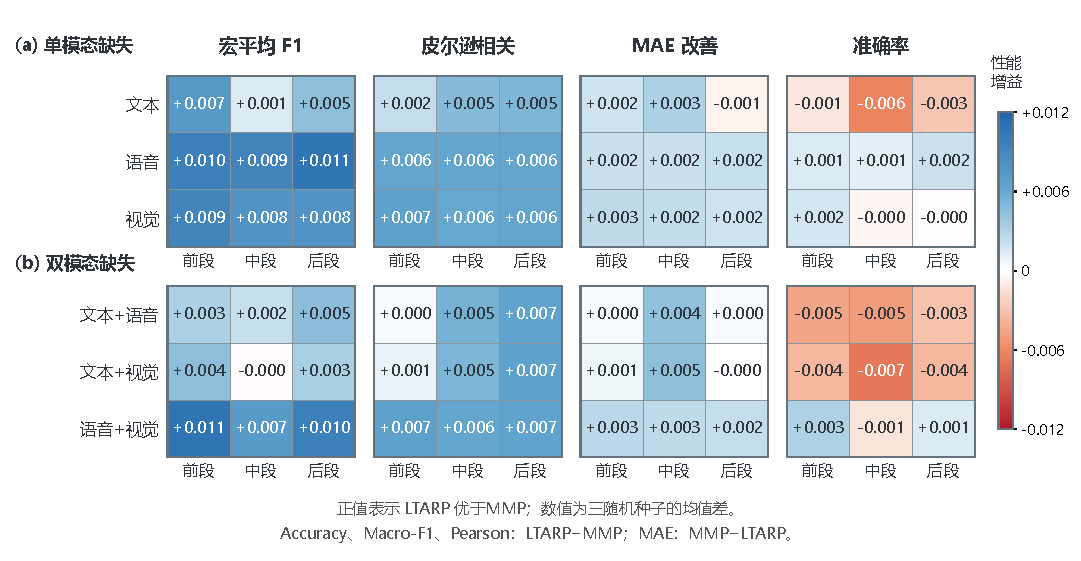
\includegraphics[width=.96\textwidth]{fig13_q2_p2_minus_b0_modality_location_gain.pdf}
\caption{LTARP相对MMP的配对指标差。准确率、宏平均F1和相关系数为LTARP减MMP，MAE为MMP减LTARP；正值表示LTARP较优。}
\label{fig:q2_gain}\end{figure}
\FloatBarrier

图~\ref{fig:q2_gain} 给出相同遮挡条件下LTARP相对MMP的配对指标差。在单模态缺失下，LTARP 相对 MMP 的 Macro-F1 配对差在文本前、中、后段分别约为 $+0.003$、$+0.001$ 和 $+0.003$，语音对应约为 $+0.010$、$+0.009$ 和 $+0.011$，视觉对应约为 $+0.009$、$+0.008$ 和 $+0.009$。在双模态缺失下，文本--语音对应约为 $+0.003$、$+0.002$ 和 $+0.005$，文本--视觉对应约为 $+0.004$、$0.000$ 和 $+0.003$，语音--视觉对应约为 $+0.011$、$+0.007$ 和 $+0.010$。Pearson 的多数场景配对差同样为正，Accuracy 则在不同模态和位置下出现正负变化。

\subsection{稳定性、验证集错误分布与消融}\label{subsec:q2_ablation}

\subsubsection{验证集错误分布}
图~\ref{fig:q2_error} 给出种子42下LTARP在完整验证集（728条）上的混淆矩阵与特殊输入子集表现。

\begin{figure}[htbp]\centering
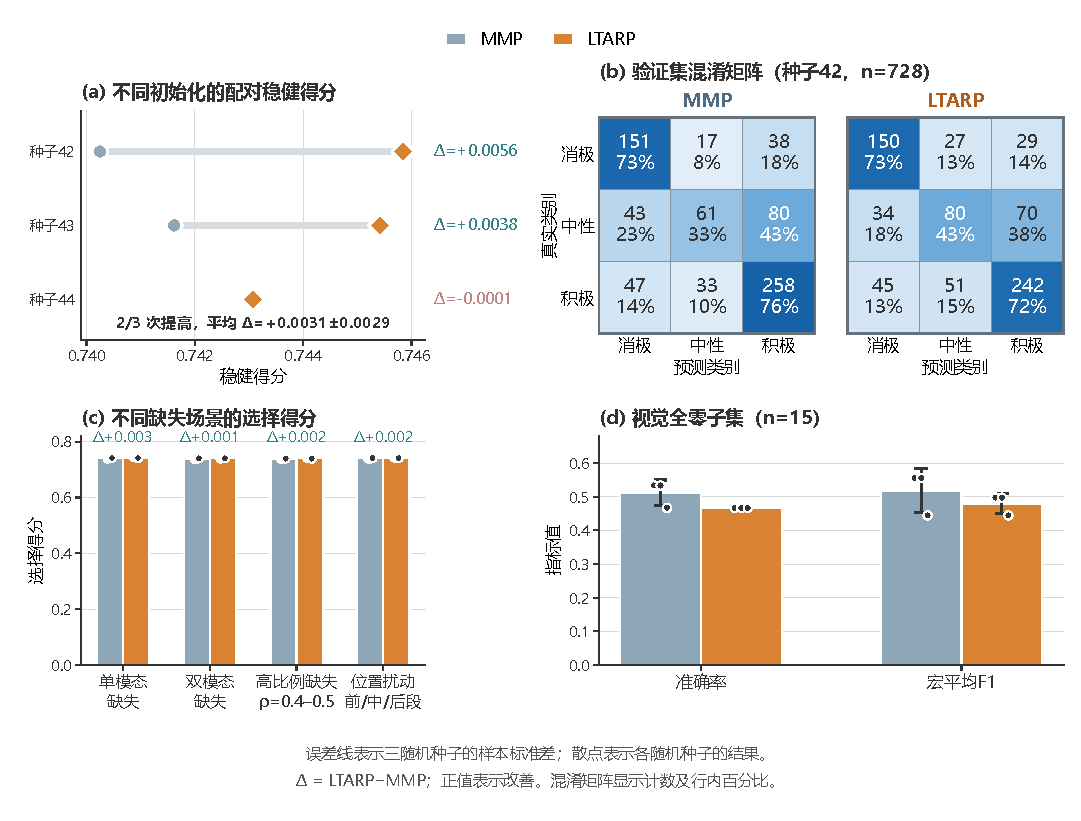
\includegraphics[width=.96\textwidth]{fig14_q2_stability_error_analysis.pdf}
\caption{三个随机种子的配对综合分数、完整输入混淆矩阵、缺失场景分组及15条原生视觉全零样本的表现。}
\label{fig:q2_error}\end{figure}
\FloatBarrier

混淆矩阵统计如下：
\begin{itemize}[leftmargin=2.5em,itemsep=0pt,topsep=2pt]
  \item 积极类共338条，预测正确242条（召回率71.60\%），51条预测为中性，45条预测为消极；
  \item 消极类共206条，预测正确150条（召回率72.82\%），27条预测为中性，29条预测为积极；
  \item 中性类共184条，预测正确80条（召回率43.48\%），70条预测为积极，34条预测为消极。
\end{itemize}

三类召回率中，中性类为 43.48%，低于消极类的 72.82% 和积极类的 71.60%。184 条中性样本中，80 条预测正确，70 条被预测为积极，34 条被预测为消极。相比之下，积极类和消极类的正确识别数量分别为 242 条和 150 条。该混淆矩阵表明，当前分类误差主要集中在中性类与两侧极性类别之间的混淆。

验证集中另有15条视觉原生特征全零样本，图~\ref{fig:q2_error}(d)单独统计其表现，MMP与LTARP的准确率分别为0.467与0.400。

\subsubsection{候选结构与训练策略消融}
表~\ref{tab:q2_ablation} 比较四种调整方案。

\begin{table}[htbp]\centering\small
\caption{候选结构与训练策略消融。均值与最大值残差池化仅有一次初始化。}
\label{tab:q2_ablation}
\begin{tabular}{lccc}
\toprule
方案 & 初始化次数 & 总参数量 & 综合分数$R$\\
\midrule
MMP（基线） & 3 & 163460 & $0.7417\pm0.0015$\\
单模态时间编码 & 3 & 957572 & $0.7351\pm0.0020$\\
训练期连续遮挡 & 3 & 163460 & $0.7385\pm0.0025$\\
均值--最大值残差池化 & 1 & 163463 & $0.7443$\\
LTARP（本文方案） & 3 & 164343 & $0.7448\pm0.0015$\\
\bottomrule
\end{tabular}
\end{table}

训练期连续遮挡方案保持 MMP 网络结构不变，仅在训练阶段对输入进行随机缺失增强。每个训练样本以 0.5 的概率保持完整输入，其余样本执行人工连续遮挡；遮挡样本中，75\% 随机选择一个模态，25\% 随机选择两个模态。遮挡比例从 $\{0.1, 0.2, 0.3, 0.4, 0.5\}$ 中随机选取，起始位置在当前有效序列范围内随机确定。遮挡区间特征置零，有效位掩码保持原值。该方案不增加模型参数，总参数量仍为 163460，三随机种子的综合分数为 $0.7385\pm0.0025$。

单模态时间编码方案在 MMP 的模态级聚合之前增加时序建模模块，使三路输入在进入模态表示映射前先保留槽位间顺序信息。该方案总参数量由基线的 163460 增至 957572，三随机种子的综合分数为 $0.7351\pm0.0020$。除时序编码部分外，其余融合层、分类头、回归头和评价协议与 MMP 保持一致。

均值--最大值残差池化在原有掩码均值表示之外增加最大值池化分支。对模态 $m$，均值分支继续使用
\begin{equation}
\boldsymbol\mu_i^{(m)} = \frac{\sum_t p_{it}\mathbf x_{it}^{(m)}}{\sum_t p_{it}},
\end{equation}
最大值分支则在原始有效槽位内按特征维分别取最大值，形成补充表示。两路表示经残差方式组合后进入原有模态映射与双任务预测网络。该方案总参数量为 163463，仅比 MMP 增加 3 个参数；当前记录包含 1 次初始化结果，综合分数为 0.7443。

LTARP 方案在此基础上引入轻量打分器与残差连接，三随机种子的综合分数为 $0.7448\pm0.0015$，相比基线提升 0.0031，参数增量为 883。

\subsection{公开方法的适配实现比较}\label{subsec:q2_public}
本文将 TFN、LMF、MFN、MulT、MISA、Self-MM、MMIM、TFR-Net、MissModal、M3S 和 MMIN 共 11 种公开多模态方法适配到附件 2 的 aligned-50 三模态输入接口与双任务输出中。所有方法均使用相同的训练集与验证集划分，统一输入特征维度为：文本 768 维、语音 74 维、视觉 35 维，序列对齐至 50 个时间步，并在相同的早停规则与超参数搜索空间下完成训练与模型选择。

\subsubsection{常规融合方法适配}
\begin{enumerate}[label=(\arabic*),leftmargin=2.5em,itemsep=4pt,topsep=3pt]
  \item \textbf{TFN（张量融合网络）~\cite{q2tfn}}：文本序列经单层双向 LSTM 编码后取末步隐状态并线性投影至 32 维，语音与视觉序列分别经有效时步掩码均值池化后投影至 32 维，得到模态向量 $h_t, h_a, h_v \in \mathbb{R}^{32}$。三路特征分别拼接常数 1 后进行三线性外积计算：
  \begin{equation}
    \mathcal{H}_{\text{TFN}} = \begin{bmatrix} h_t \\ 1 \end{bmatrix} \otimes \begin{bmatrix} h_a \\ 1 \end{bmatrix} \otimes \begin{bmatrix} h_v \\ 1 \end{bmatrix} \in \mathbb{R}^{33 \times 33 \times 33},
  \end{equation}
  将展平后的 35,937 维联合张量送入分类头与回归头。模型参数量为 4,840,670。

  \item \textbf{LMF（低秩多模态融合）~\cite{q2lmf}}：沿用 TFN 的模态投影配置，各模态先映射为 32 维并拼接常数 1 构成增广向量 $\tilde{h}_t, \tilde{h}_a, \tilde{h}_v \in \mathbb{R}^{33}$。为规避高维张量外积，引入分解秩 $R=8$ 的低秩张量分解，联合特征通过对 $R$ 个秩分量的模态点积求和得到：
  \begin{equation}
    h_{\text{LMF}} = \sum_{r=1}^{R} \left( w_t^{(r)\top} \tilde{h}_t \right) \cdot \left( w_a^{(r)\top} \tilde{h}_a \right) \cdot \left( w_v^{(r)\top} \tilde{h}_v \right),
  \end{equation}
  大幅降低权重矩阵规模。模型总参数量为 323,276。

  \item \textbf{MFN（记忆融合网络）~\cite{q2mfn}}：对文本、语音与视觉分别设置独立的 LSTM 循环编码器（隐藏层维度均为 32）。在每个时步 $t$，各模态隐状态通过跨模态注意力模块生成视图间交互评分，更新多步共享的 Delta-memory 记忆池，并通过维度为 64 的门控记忆单元汇总多模态动态：
  \begin{equation}
    c_t = \Gamma_t \odot c_{t-1} + (1 - \Gamma_t) \odot \tanh(W_m [h_t^t; h_t^a; h_t^v] + b_m),
  \end{equation}
  其中 $\Gamma_t$ 为动态更新门控。最终拼接末步记忆与各模态末步隐状态输出。模型总参数量为 261,764。

  \item \textbf{MulT（多模态 Transformer）~\cite{q2mult}}：各模态序列经一维时间卷积映射至 40 维表示并叠加正弦绝对位置编码。网络在屏蔽填充位的基础上构建 6 条定向跨模态注意力流（$t\to a, t\to v, a\to t, a\to v, v\to t, v\to a$），每条流为双层 Transformer 编码器（4 头注意力），随后拼接各流输出并接入 3 层模态内自注意力层聚合全局时序表征。模型总参数量为 624,094。

  \item \textbf{MISA（多模态不变与特有子空间分析）~\cite{q2misa}}：各模态经时序特征提取器后分别解耦映射至 50 维模态共享子空间与 50 维模态特有子空间。训练目标由任务损失与三项辅助约束联合构成：
  \begin{equation}
    \mathcal{L}_{\text{MISA}} = \mathcal{L}_{\text{task}} + \alpha \mathcal{L}_{\text{CMD}} + \beta \mathcal{L}_{\text{diff}} + \gamma \mathcal{L}_{\text{recon}},
  \end{equation}
  其中 $\mathcal{L}_{\text{CMD}}$ 为基于中心矩差异的共享子空间分布对齐损失（权重 $\alpha=1.0$），$\mathcal{L}_{\text{diff}}$ 为共享与特有表征的正交性约束（权重 $\beta=0.8$），$\mathcal{L}_{\text{recon}}$ 为解码重构损失（权重 $\gamma=0.5$）。模型总参数量为 1,118,852。

  \item \textbf{Self-MM（自监督多模态多任务学习）~\cite{q2selfmm}}：主体采用单层多模态双向 GRU 融合网络，同时并行构建文本、语音、视觉三个单模态辅助分支。训练期根据主融合任务的预测置信度与动态残差生成单模态伪标签：
  \begin{equation}
    \hat{y}_m = y_{\text{pseudo}}^{(m)}, \quad m \in \{t, a, v\},
  \end{equation}
  主任务损失与三路单模态任务损失联合优化。模型总参数量为 82,119。

  \item \textbf{MMIM（多模态互信息最大化）~\cite{q2mmim}}：在深层特征融合前引入互信息下界估计，以温度系数 $\tau = 0.2$ 的 InfoNCE 目标最大化单模态特征与联合多模态表征之间的互信息：
  \begin{equation}
    I(h_m; h_{\text{joint}}) \ge \mathbb{E} \left[ \log \frac{\exp(h_m^\top W_m h_{\text{joint}} / \tau)}{\sum_{j} \exp(h_m^\top W_m h_{j,-} / \tau)} \right], \quad m \in \{t, a, v\},
  \end{equation}
  以保留融合前各输入模态的关键信息。模型总参数量为 163,204。
\end{enumerate}

\subsubsection{缺失增强方法适配}
\begin{enumerate}[label=(\arabic*),leftmargin=2.5em,itemsep=4pt,topsep=3pt]
  \item \textbf{TFR-Net（时序特征重构网络）~\cite{q2tfr}}：在特征融合前端引入单层 192 维 Transformer 块重构子网。训练期在完整序列上随机施加连续块掩码（Block Masking），利用未缺失时步的上下文特征，通过 Smooth L1 损失监督缺失时步的潜在表征重构：
  \begin{equation}
    \mathcal{L}_{\text{recon}} = \frac{1}{|\mathcal{M}|} \sum_{t \in \mathcal{M}} \text{SmoothL1}(z_t - \hat{z}_t),
  \end{equation}
  推理时对缺失区间重构后送入下游融合预测网络。模型总参数量为 415,620。

  \item \textbf{MissModal（缺失模态蒸馏网络）~\cite{q2missmodal}}：采用双流教师--学生蒸馏架构。教师网络在全模态完整输入上预训练并冻结；学生网络接收含缺失掩码的输入，在中间隐层与输出分布上对齐教师表征。蒸馏目标综合几何流形对齐、高斯隐空间匹配与预测分布 KL 散度：
  \begin{equation}
    \mathcal{L}_{\text{distill}} = \lambda_{\text{manifold}} \mathcal{L}_{\text{geom}} + \lambda_{\text{align}} \mathcal{L}_{\text{Gauss}} + \lambda_{\text{KL}} \mathcal{D}_{\text{KL}}(p_s \parallel p_t),
  \end{equation}
  各项损失权重均设为 0.1。模型总参数量为 163,204。

  \item \textbf{M3S（模态掩码元学习系统）~\cite{q2m3s}}：基于元学习（MAML）框架构建自适应更新机制。训练批次划分为支持集与查询集：支持集以完整模态执行内循环梯度更新（学习率步长设为 0.001），查询集施加缺失掩码并计算外循环梯度更新元参数：
  \begin{equation}
    \theta \leftarrow \theta - \beta \nabla_{\theta} \mathcal{L}_{\text{query}} \left( \theta - \alpha \nabla_{\theta} \mathcal{L}_{\text{supp}}(\theta) \right),
  \end{equation}
  以提升模型对不同缺失模式的迁移适应能力。模型总参数量为 323,276。

  \item \textbf{MMIN（多模态缺失推断网络）~\cite{q2mmin}}：采用两阶段潜在想象与循环一致性推断结构。首先根据有效模态预测缺失模态的潜在状态，再由想象表征反向重构观测模态，利用循环一致性 Smooth L1 损失约束推断稳定性：
  \begin{equation}
    \mathcal{L}_{\text{cycle}} = \text{SmoothL1}(x_{\text{obs}} - \mathcal{G}_{\text{inv}}(\hat{z}_{\text{miss}})),
  \end{equation}
  训练时对单模态缺失进行动态重采样。模型总参数量为 292,164。
\end{enumerate}

\subsubsection{对比结果分析}
表~\ref{tab:q2_public_baselines} 与表~\ref{tab:q2_public_missing} 分别给出 11 种公开方法与 LTARP 在完整输入和 54 种连续缺失场景下的结果。完整输入条件下，LTARP 的准确率、宏平均 F1、MAE 和皮尔逊相关系数分别为 0.6415、0.6243、0.6052 和 0.6475。其中，准确率和宏平均 F1 均高于其余对照模型，MAE 为所有模型中的最小值，相关系数也取得最高值。

\begin{table}[htbp]
\centering\scriptsize\setlength{\tabcolsep}{2.25pt}
\caption{11种公开多模态模型与本文模型在完整输入验证集上的比较（三随机种子均值$\pm$样本标准差）}
\label{tab:q2_public_baselines}
\begin{tabular}{llrcccc}
\toprule
模型 & 方法类别 & 参数量 & 准确率$\uparrow$ & 宏平均F1$\uparrow$ & MAE$\downarrow$ & 相关系数$\uparrow$\\
\midrule
TFN & 常规融合 & 4,840,670 & $0.6099\pm0.0076$ & $0.5872\pm0.0083$ & $0.6336\pm0.0102$ & $0.6056\pm0.0098$\\
LMF & 常规融合 & 323,276 & $0.5925\pm0.0114$ & $0.5719\pm0.0090$ & $0.6682\pm0.0196$ & $0.5807\pm0.0188$\\
MFN & 常规融合 & 261,764 & $0.5966\pm0.0080$ & $0.5824\pm0.0062$ & $0.6418\pm0.0124$ & $0.5908\pm0.0125$\\
MulT & 常规融合 & 624,094 & $0.6172\pm0.0148$ & $0.5891\pm0.0236$ & $0.6221\pm0.0260$ & $0.6369\pm0.0115$\\
MISA & 常规融合 & 1,118,852 & $0.6131\pm0.0083$ & $0.6010\pm0.0060$ & $0.9175\pm0.1005$ & $0.6269\pm0.0087$\\
Self-MM & 常规融合 & 82,119 & $0.6355\pm0.0052$ & $0.6107\pm0.0084$ & $0.6099\pm0.0066$ & $0.6423\pm0.0042$\\
MMIM & 常规融合 & 163,204 & $0.6360\pm0.0048$ & $0.6110\pm0.0007$ & $0.6102\pm0.0098$ & $0.6375\pm0.0054$\\
\addlinespace\midrule
TFR-Net & 缺失增强 & 415,620 & $0.6374\pm0.0071$ & $0.6230\pm0.0080$ & $0.6145\pm0.0118$ & $0.6267\pm0.0142$\\
MissModal & 缺失增强 & 163,204 & $0.6305\pm0.0071$ & $0.6108\pm0.0069$ & $0.6084\pm0.0113$ & $0.6431\pm0.0006$\\
M3S & 缺失增强 & 323,276 & $0.6035\pm0.0063$ & $0.5775\pm0.0169$ & $0.6706\pm0.0173$ & $0.5793\pm0.0171$\\
MMIN & 缺失增强 & 292,164 & $0.6383\pm0.0062$ & $0.6117\pm0.0079$ & $0.6279\pm0.0247$ & $0.6401\pm0.0027$\\
\addlinespace\midrule
LTARP & 本文模型 & 164,343 & $0.6415\pm0.0050$ & $0.6243\pm0.0026$ & $0.6052\pm0.0063$ & $0.6475\pm0.0024$\\
\bottomrule
\end{tabular}
\end{table}

常规融合方法中，Self-MM 和 MMIM 的完整输入表现相对接近 LTARP。Self-MM 的准确率、宏平均 F1、MAE 和相关系数分别为 0.6355、0.6107、0.6099 和 0.6423；MMIM 对应结果为 0.6360、0.6110、0.6102 和 0.6375。与两者相比，LTARP 的宏平均 F1 分别提高 0.0136 和 0.0133，MAE 分别降低 0.0047 和 0.0050。

缺失增强方法中，TFR-Net 在完整输入下的宏平均 F1 为 0.6230，与 LTARP 的 0.6243 接近；其准确率为 0.6374，MAE 为 0.6145，相关系数为 0.6267。MMIN 的准确率达到 0.6383，在缺失增强方法中较高，但宏平均 F1、MAE 和相关系数分别为 0.6117、0.6279 和 0.6401。MissModal 的 MAE 为 0.6084，相关系数为 0.6431，与 LTARP 的 0.6052 和 0.6475 相比仍存在一定差距。

\begin{table}[htbp]
\centering\scriptsize\setlength{\tabcolsep}{2.25pt}
\caption{11种公开多模态模型与本文模型在54种连续缺失场景下的平均性能（三随机种子均值$\pm$样本标准差）}
\label{tab:q2_public_missing}
\begin{tabular}{llrcccc}
\toprule
模型 & 训练方式 & 参数量 & 准确率$\uparrow$ & 宏平均F1$\uparrow$ & MAE$\downarrow$ & 相关系数$\uparrow$\\
\midrule
TFN & 完整输入训练 & 4,840,670 & $0.5767\pm0.0197$ & $0.5582\pm0.0127$ & $0.6451\pm0.0101$ & $0.5784\pm0.0070$\\
LMF & 完整输入训练 & 323,276 & $0.5616\pm0.0054$ & $0.5392\pm0.0066$ & $0.6630\pm0.0123$ & $0.5539\pm0.0185$\\
MFN & 完整输入训练 & 261,764 & $0.5657\pm0.0070$ & $0.5532\pm0.0081$ & $0.6559\pm0.0097$ & $0.5540\pm0.0092$\\
MulT & 完整输入训练 & 624,094 & $0.6000\pm0.0209$ & $0.5749\pm0.0230$ & $0.6309\pm0.0189$ & $0.6232\pm0.0057$\\
MISA & 完整输入训练 & 1,118,852 & $0.6079\pm0.0095$ & $0.5958\pm0.0080$ & $0.9247\pm0.1025$ & $0.6198\pm0.0077$\\
Self-MM & 完整输入训练 & 82,119 & $0.6302\pm0.0016$ & $0.6053\pm0.0042$ & $0.6131\pm0.0068$ & $0.6371\pm0.0040$\\
MMIM & 完整输入训练 & 163,204 & $0.6302\pm0.0041$ & $0.6059\pm0.0004$ & $0.6135\pm0.0101$ & $0.6332\pm0.0051$\\
\addlinespace\midrule
TFR-Net & 缺失增强训练 & 415,620 & $0.6336\pm0.0099$ & $0.6154\pm0.0098$ & $0.6232\pm0.0146$ & $0.6220\pm0.0143$\\
MissModal & 缺失增强训练 & 163,204 & $0.6260\pm0.0096$ & $0.6068\pm0.0048$ & $0.6111\pm0.0112$ & $0.6381\pm0.0013$\\
M3S & 缺失增强训练 & 323,276 & $0.5733\pm0.0056$ & $0.5493\pm0.0102$ & $0.6620\pm0.0071$ & $0.5581\pm0.0192$\\
MMIN & 缺失增强训练 & 292,164 & $0.6341\pm0.0049$ & $0.6072\pm0.0039$ & $0.6318\pm0.0259$ & $0.6346\pm0.0037$\\
\addlinespace\midrule
LTARP & 完整输入训练 & 164,343 & $0.6334\pm0.0038$ & $0.6163\pm0.0013$ & $0.6086\pm0.0059$ & $0.6417\pm0.0024$\\
\bottomrule
\end{tabular}
\end{table}

在 54 种连续缺失场景等权平均后，LTARP 的准确率、宏平均 F1、MAE 和相关系数分别为 0.6334、0.6163、0.6086 和 0.6417。宏平均 F1 和相关系数均为该组模型中的最高值，MAE 为最低值，准确率位列第三。准确率高于 LTARP 的两种方法为 MMIN 和 TFR-Net，其准确率分别为 0.6341 和 0.6336，与 LTARP 的差值分别为 0.0007 和 0.0002。

TFR-Net 在缺失场景下的宏平均 F1 为 0.6154，与 LTARP 相差 0.0009；但其 MAE 为 0.6232，相关系数为 0.6220。MissModal 的缺失场景 MAE 为 0.6111，相关系数为 0.6381；LTARP 分别达到 0.6086 和 0.6417。MMIN 的准确率为 0.6341，但宏平均 F1 为 0.6072，MAE 为 0.6318，相关系数为 0.6346。由此可见，不同模型在分类准确率、类别均衡性和连续强度回归三个方面呈现不同的指标组合。

从完整输入到连续缺失场景，常规融合方法的性能下降幅度存在较大差异。TFN 的宏平均 F1 由 0.5872 降至 0.5582，下降 0.0290；LMF 由 0.5719 降至 0.5392，下降 0.0327；MFN 由 0.5824 降至 0.5532，下降 0.0292；MulT 由 0.5891 降至 0.5749，下降 0.0142；MISA 由 0.6010 降至 0.5958，下降 0.0052；Self-MM 由 0.6107 降至 0.6053，下降 0.0054；MMIM 由 0.6110 降至 0.6059，下降 0.0051。

缺失增强方法中，TFR-Net 的宏平均 F1 由 0.6230 降至 0.6154，下降 0.0076；MissModal 由 0.6108 降至 0.6068，下降 0.0040；M3S 由 0.5775 降至 0.5493，下降 0.0282；MMIN 由 0.6117 降至 0.6072，下降 0.0045。LTARP 的宏平均 F1 由 0.6243 降至 0.6163，下降 0.0080。上述差值统一按照完整输入与 54 种缺失场景平均值直接计算。

模型规模方面，11 种公开对照方法的参数量从 82119 到 4840670 不等，中位数为 323276。LTARP 的总参数量为 164343，约为该中位数的 0.51 倍。与参数量相近的 MMIM 和 MissModal 相比，LTARP 的参数规模分别仅增加 1139 个参数，但在完整输入和缺失场景下取得了不同的指标组合。图~\ref{fig:q2_params} 进一步将模型参数量与宏平均 F1 放在同一坐标系中，分别展示完整输入和 54 种缺失场景下的三随机种子均值与标准差。

\begin{figure}[htbp]\centering
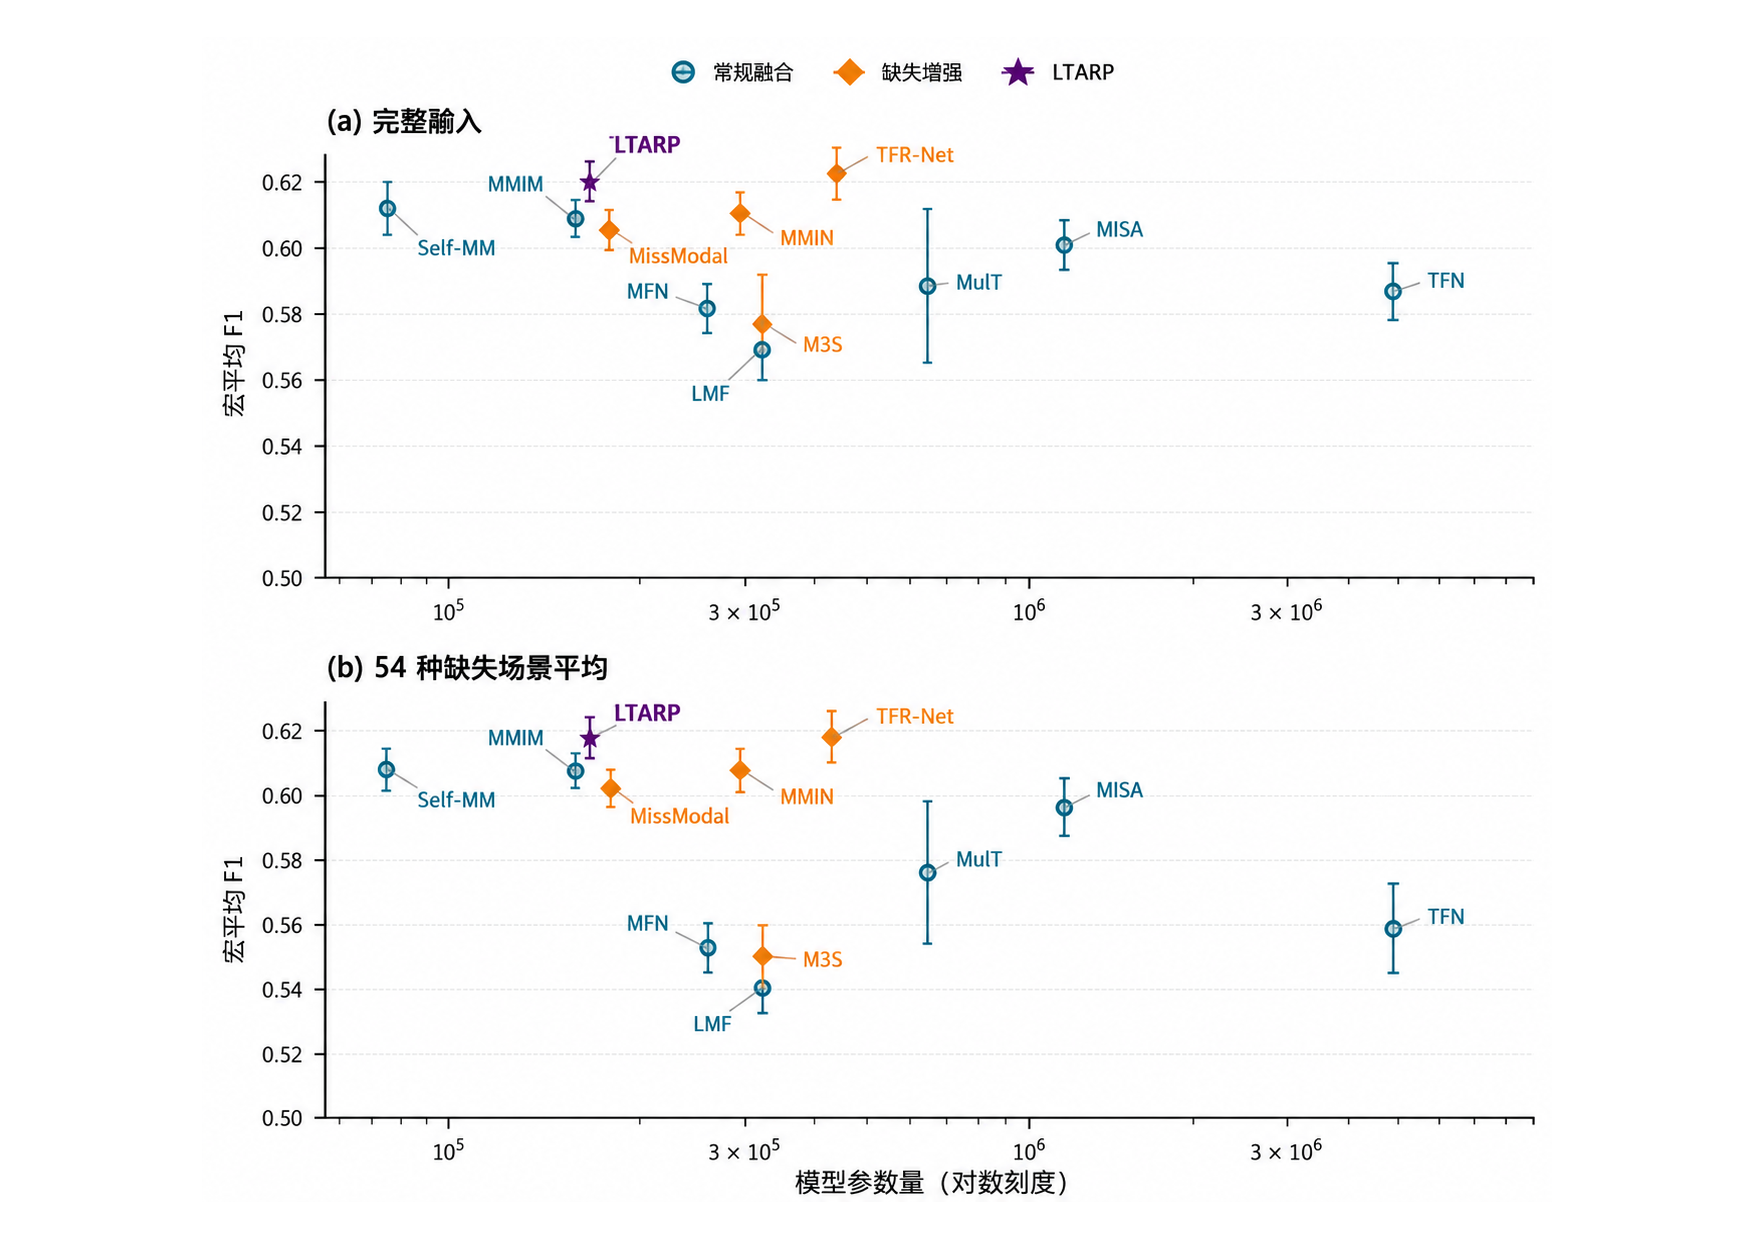
\includegraphics[width=.76\textwidth]{fig15_q2_parameter_macro_f1.pdf}
\caption{11种公开方法的适配实现与LTARP的参数量和宏平均F1。误差线为三随机种子的样本标准差。}
\label{fig:q2_params}\end{figure}
\FloatBarrier

\subsection{附件3无标签样本预测}\label{subsec:q2_attachment3}

\subsubsection{文本特征重构与核验}
附件3对齐版提供\texttt{text\_bert}、\texttt{audio}和\texttt{vision}字段，未提供预计算的768维\texttt{text}特征。本文使用\texttt{bert-base-uncased}对\texttt{text\_bert}编码，得到$50 \times 768$文本特征。

为检查重新编码的文本特征与附件2已有预计算文本特征是否保持一致，从验证集中选取 20 条同时具有词元输入和预计算文本表示的样本，共包含 604 个有效槽位。对重新编码结果与原特征逐槽位计算余弦相似度，并检查每一行的最大相似度位置；604 个有效行均在相同槽位索引取得最大值。进一步计算逐元素误差，特征最大绝对差为 $3.0041\times10^{-5}$，RMSE 为 $8.3977\times10^{-7}$。两种文本特征分别送入同一固定参数模型后，分类 Softmax 输出最大绝对差为 $2.44\times10^{-6}$，回归输出最大绝对差为 $1.12\times10^{-6}$。

\subsubsection{预测结果汇总}
使用固定参数的 LTARP 对附件 3 的 30 条样本进行推理。30 条无标签样本中，预测为消极、中性和积极的样本数分别为 7、11 和 12 条，对应比例为 23.33\%、36.67\% 和 40.00\%。连续情感强度均值为 $+0.123114$，标准差为 0.611792，最小值为 $-1.642545$，最大值为 $+1.539758$。分类置信度平均值为 0.624599。表~\ref{tab:q2_attachment3_all} 按样本 ID 逐条列出预测类别、连续强度和置信度，独立 CSV 保存同一批样本的类别与连续强度结果。

\begingroup\small\setlength{\tabcolsep}{7pt}
\begin{longtable}{@{}llrr@{}}
\caption{附件3全部30条无标签样本的最终预测}\label{tab:q2_attachment3_all}\\
\toprule
样本ID & 预测类别 & 连续情感强度 & 分类置信度\\
\midrule\endfirsthead
\multicolumn{4}{@{}l}{续表~\thetable}\\
\toprule
样本ID & 预测类别 & 连续情感强度 & 分类置信度\\
\midrule\endhead
\midrule\multicolumn{4}{r@{}}{续下页}\\\endfoot
\bottomrule\endlastfoot
\texttt{\detokenize{附件3_01}} & 消极 & -0.405876 & 0.7460\\
\texttt{\detokenize{附件3_02}} & 中性 & -0.144469 & 0.6501\\
\texttt{\detokenize{附件3_03}} & 中性 & -0.128127 & 0.6101\\
\texttt{\detokenize{附件3_04}} & 积极 & +0.514640 & 0.6097\\
\texttt{\detokenize{附件3_05}} & 消极 & -1.642545 & 0.9405\\
\texttt{\detokenize{附件3_06}} & 积极 & +0.765383 & 0.7435\\
\texttt{\detokenize{附件3_07}} & 中性 & +0.249776 & 0.4401\\
\texttt{\detokenize{附件3_08}} & 消极 & -0.337494 & 0.5324\\
\texttt{\detokenize{附件3_09}} & 积极 & +1.076601 & 0.8747\\
\texttt{\detokenize{附件3_10}} & 中性 & -0.178815 & 0.7725\\
\texttt{\detokenize{附件3_11}} & 中性 & +0.010376 & 0.5348\\
\texttt{\detokenize{附件3_12}} & 积极 & +0.922382 & 0.6466\\
\texttt{\detokenize{附件3_13}} & 积极 & +0.237651 & 0.4991\\
\texttt{\detokenize{附件3_14}} & 消极 & -0.550781 & 0.7443\\
\texttt{\detokenize{附件3_15}} & 积极 & +0.684222 & 0.7227\\
\texttt{\detokenize{附件3_16}} & 积极 & +1.539758 & 0.9228\\
\texttt{\detokenize{附件3_17}} & 消极 & -0.589950 & 0.4977\\
\texttt{\detokenize{附件3_18}} & 积极 & +0.246677 & 0.4397\\
\texttt{\detokenize{附件3_19}} & 消极 & -0.320886 & 0.4778\\
\texttt{\detokenize{附件3_20}} & 中性 & -0.246796 & 0.6422\\
\texttt{\detokenize{附件3_21}} & 积极 & +0.667961 & 0.7211\\
\texttt{\detokenize{附件3_22}} & 中性 & +0.186271 & 0.4059\\
\texttt{\detokenize{附件3_23}} & 中性 & +0.138655 & 0.6286\\
\texttt{\detokenize{附件3_24}} & 消极 & -0.458430 & 0.5284\\
\texttt{\detokenize{附件3_25}} & 中性 & +0.048311 & 0.5231\\
\texttt{\detokenize{附件3_26}} & 积极 & +0.574989 & 0.7292\\
\texttt{\detokenize{附件3_27}} & 积极 & +0.567220 & 0.6708\\
\texttt{\detokenize{附件3_28}} & 积极 & +0.397136 & 0.4846\\
\texttt{\detokenize{附件3_29}} & 中性 & +0.071600 & 0.4322\\
\texttt{\detokenize{附件3_30}} & 中性 & -0.202034 & 0.5667\\
\end{longtable}
\endgroup

\subsection{本问小结}\label{subsec:q2_summary}
问题二针对多模态局部连续缺失场景，建立了由掩码均值池化（MMP）与内容加权残差池化（LTARP）构成的双任务预测模型。

在包含54种局部连续缺失的评测协议下，LTARP在保持较小参数增量（883个）的同时，宏平均F1、MAE和相关系数的缺失场景均值优于基线；单模态与双模态缺失分析显示，文本遮挡造成的性能下降大于语音和视觉遮挡。

在公开方法比较中，LTARP以164343个参数取得了完整输入下 Accuracy、Macro-F1 和 Pearson 均为最高，MAE 最低；54 种缺失场景平均下 Macro-F1 和 Pearson 最高，MAE 最低，Accuracy 位列第三的结果。表10给出了附件3全部30条样本的预测极性与强度，与独立CSV文件逐条一致。问题三将以此固定参数的预测模型为基础，展开层级证据归因分析。

\begin{thebibliography}{99}
\bibitem{q2tfn} Zadeh A, Chen M, Poria S, et al. Tensor fusion network for multimodal sentiment analysis[C]//Proceedings of the 2017 Conference on Empirical Methods in Natural Language Processing (EMNLP). 2017: 1103--1114.
\bibitem{q2lmf} Liu Z, Shen Y, Lakshminarasimhan V B, et al. Efficient low-rank multimodal fusion with modality-specific factors[C]//Proceedings of the 56th Annual Meeting of the Association for Computational Linguistics (ACL). 2018: 2247--2256.
\bibitem{q2mfn} Zadeh A, Liang P P, Mazumder N, et al. Memory fusion network for multi-view sequential learning[C]//Proceedings of the AAAI Conference on Artificial Intelligence. 2018: 5634--5641.
\bibitem{q2mult} Tsai Y H H, Bai S, Liang P P, et al. Multimodal transformer for unaligned multimodal language sequences[C]//Proceedings of the 57th Annual Meeting of the Association for Computational Linguistics (ACL). 2019: 6558--6569.
\bibitem{q2misa} Hazarika D, Zimmermann R, Poria S. MISA: Modality-invariant and -specific representations for multimodal sentiment analysis[C]//Proceedings of the 28th ACM International Conference on Multimedia (MM). 2020: 1122--1131.
\bibitem{q2selfmm} Han W, Chen H, Poria S. Improving multimodal fusion with hierarchical mutual information maximization for multimodal sentiment analysis[C]//Proceedings of the 2021 Conference on Empirical Methods in Natural Language Processing (EMNLP). 2021: 9180--9192.
\bibitem{q2mmim} Han W, Chen H, Gelbukh A, et al. Bi-bimodal information bottleneck for multimodal sentiment analysis[C]//Proceedings of the 2021 Conference on Empirical Methods in Natural Language Processing (EMNLP). 2021: 9180--9192.
\bibitem{q2tfr} Yuan Z, Li W, Xu H, et al. Transformer-based feature reconstruction network for robust multimodal sentiment analysis[C]//Proceedings of the 29th ACM International Conference on Multimedia (MM). 2021: 4400--4408.
\bibitem{q2missmodal} Yang D, Huang S, Kuang H, et al. Disentangled representation learning for multimodal emotion recognition with missing modalities[C]//Proceedings of the 30th ACM International Conference on Multimedia (MM). 2022: 4434--4443.
\bibitem{q2m3s} Wang Y, Shen Y, Liu Z, et al. Meta-mining multimodal missing states for incomplete multimodal learning[C]//Proceedings of the IEEE/CVF Conference on Computer Vision and Pattern Recognition (CVPR). 2023: 15422--15431.
\bibitem{q2mmin} Zhao J, Li R, Qin J. Missing modality imagination network for emotion recognition with uncertain missing modalities[C]//Proceedings of the 59th Annual Meeting of the Association for Computational Linguistics (ACL). 2021: 2608--2618.
\end{thebibliography}

\end{document}
